\documentclass[a4,center,fleqn]{NAR}

% Enter dates of publication
\copyrightyear{2008}
\pubdate{31 July 2009}
\pubyear{2009}
\jvolume{37}
\jissue{12}

%\articlesubtype{This is the article type (optional)}

\begin{document}

\title{Faithful short-read mapping with Sesame}

\author{%
Ruggero Cortini\,$^{1,\text{\#}}$,
Eduard Valera Zorita\,$^{1,\text{\#}}$,
Guillaume J. Filion\,$^{1,2,3}$
\footnote{To whom correspondence should be addressed.
Email: guillaume.filion@gmail.com}}

\address{%
$^{1}$Center for Genomic Regulation (CRG), The Barcelona Institute
of Science and Technology, Dr. Aiguader 88, Barcelona 08003, Spain;
$^{2}$University Pompeu Fabra (UPF), Barcelona, Spain;
$^{3}$present address: Department of Biological Sciences, University
of Toronto Scarborough, Toronto, ON, Canada; $^{\text{\#}}$ equal
contributions.}
% Affiliation must include:
% Department name, institution name, full road and district address,
% state, Zip or postal code, country

\history{%
Received January 1, 2009;
Revised February 1, 2009;
Accepted March 1, 2009}

\maketitle

\begin{abstract}
Abstract will come later.
\end{abstract}


\section{Introduction}

High throughput DNA sequencing is now a standard technology in the
academia and in the industry, with countless applications in diagnosis,
forensics, surveillance and research \cite{1}. The Illumina short-read
technology currently dominates the market of DNA sequencing, making the
associated software an important target for optimization.

The standard way to identify a read is to map it to a known reference
sequence, typically a genome. Work on short-read mappers has been
traditionally focused on improving the speed, reducing the memory
footprint and increasing the accuracy. Another important focus has been to
develop variations to address the actual needs of the user, as different
problems often entail different read types (e.g., compare CHiP-seq and
Hi-C).

Meanwhile, progress has been more limited on another aspect of the mapping
process: \emph{faithfulness}. Mapping algorithms are heuristics, so there
is always a chance that the proposed location of a read is wrong.
Faithfulness is the capacity to correctly estimate this probability.
Importantly, one can reduce the probability of errors without having to
measure it, so accuracy and faithfulness are usually unrelated.

The importance of faithfulness is recognized in the specifications of the
SAM format \cite{1} that include a \emph{mapping quality} field. The
standard defines it as $-10 \cdot \log_{10}Pr$\{mapping position is
wrong\}, i.e. quality 20 stands for one error in 100 reads, quality 30 for
one error in 1000 reads \textit{etc}. Some mappers disregard the standard
and use a qualitative scale instead (e.g., STAR) while some others do not
compute a mapping quality (e.g., GEM). As for the mappers that do comply
with the SAM standard, the scores are undocumented, variable between
mappers and versions, spreading puzzlement and frustration in the
community\footnote{http://www.acgt.me/blog/2015/3/17/more-madness-with-mapq-scores-aka-why-bioinformaticians-hate-poor-and-incomplete-software-documentation}.

The source of the issue is that there is presently no known method to
properly estimate mapping quality. In other words, the the faithful
mapping problem has no accepted solution. Yet, this is an important
challenge for the following reasons:
$i$ in many applications it is essential to know the risk associated with
every read (e.g., contaminated material such as ancient DNA);
$ii$ a mapper is easier to use if error rates are what they claim to
be;
$iii$ good calibrations open opportunities to improve the speed-accuracy
tradeoff.

We recently proposed a strategy to compute the error rate of different
seeding strategies used in short-read mappers \cite{1}. This strategy
borrows some basic concepts from analytic combinatorics \cite{1} to
develop a formal computation framework. Here we present a C implementation
of this framework in a library called Sesame. We also develop a
statistical method to estimate the parameters required to compute seeding
probabilities. We demonstrate the feasibility of our approach by
developing a naive mapper based on Sesame. Not only is this mapper
faithful, but it also reveals the existence of ``super reads'' that can be
mapped with much higher confidence than was previously thought possible.

\begin{align*}
&\mathrm{Ascorbate} + \mathrm{EDTA} \cdot \mathrm{Fe}^{3+} \to
\hbox{Oxidized ascorbate}
\\
&\mathrm{EDTA} \cdot \mathrm{Fe}^{2+} + \mathrm{H}_2
\mathrm{O}_2 \to
\mathrm{EDTA} \cdot \mathrm{Fe}^{3+} + \cdot
\mathrm{OH} + \mathrm{OH}^-
\end{align*}

% **************************************************************
% Keep this command to avoid text of first page running into the
% first page footnotes
\enlargethispage{-65.1pt}
% **************************************************************

Text. Text. Text. Text. Text. Text. Text. Text. Text \cite{2,3}.
Text. Text. Text. Text. Text. Text. Text. Text. Text \cite{4}.


\section{MATERIALS AND METHODS}

\subsection{Materials subsection one}

Text. Text. Text. Text. Text. Text. Text. Text. Text. Text. Text.
Text. Text. Text. Text. Text. Text. Text. Text. Text. Text.


\subsubsection{Materials subsubsection one.}

Text. Text. Text. Text. Text. Text. Text. Text. Text. Text. Text.
Text. Text. Text. Text. Text. Text. Text. Text. Text. Text. Text.
Text. Text. Text. Text:
\begin{align}
\mathrm{LD}^r = \frac{\mathrm{LD}}{A_\mathrm{iso}}
= 1.5 S \left( 3 \cos^2 \alpha_i - 1 \right)
\end{align}


\subsection{Materials subsection two}


Text. Text. Text. Text. Text. Text. Text.
\begin{equation*}
\mathrm{LD} \left( t \right) =
\sum\limits_i
a_i \exp \left( \frac{-t}{\tau_i} \right)
\end{equation*}
Text. Text. Text. Text. Text. Text. Text. Text. Text. Text. Text.


\section{RESULTS}

\subsection{The Sesame library}

% !! IMPORTANT !! %
% Say something about the seeds. In particular, it is important to
% mention that we do not do spaced seeds.

We wrote a C library to compute seeding probabilities from the theoretical
results presented in \cite{1}. Briefly, the strategy was to represent
reads and off-target sequences in a custom combinatorial alphabet, specify
the generating functions of basic words and define a language based on a
transfer matrix. The powers of the transfer matrix contain the generating
functions of the reads of interest, from which we can extract their
probability of ocurrence.

The probability that a read contains a seed depends on the problem and on
the read. Sesame computes seeding probabilities from five user-specified
parameters. The problem-specific parameters are known to the user and
consist of the read length $k$, the error rate $p$ and the minimum seed
size $\gamma$. The read-specific parameters are unknown to the user and
consist of the number of duplicates of the target $N$, and their average
sequence divergence $\mu$. We will explain below how to estimate them in
practice.

The Sesame library was built for performance so that it can be integrated
in mapping frameworks. This means that computations are performed only
once for a given set of parameters and memoized for later retrieval. The
parameters $k$, $p$ and $\gamma$ are constant throughout the sequencing
run, but $N$ and $\mu$ must be computed for every read. By default, Sesame
collapses the $(N, \mu)$ pairs to a coarse grid of $15 \times 3=45$
values. Computing all 45 values takes a few minutes on modern hardware,
which is negligible compared to mapping a sequencing run with several
million reads. In addition, the computed values can be saved on disk for
reuse in later runs. The user interface and available options are further
described on the main page of the repository.


\subsection{Comparing seeding strategies}

The seeding step is an essential part of read mapping. Choosing an
appropriate strategy is important, but this is usually based on limited
testing. With accurate seeding probabilities, it is possible to compare
the merits of different seeding strategies, which can be useful for
choosing a seed type or a minimum seed length.

As an example, we compare the default strategies of BWA and Bowtie2 at 1\%
sequencing error. Note that both mappers use advanced methods to refine
the seeding heuristic, so the comparison does not reflect their
performance. It is nevertheless useful to give a baseline for the
potential of each strategy. The default strategy of BWA it to use MEM
seeds of minimum size 19; that of Bowtie2 is to use seeds of size 16 every
ten nucleotides (referred to here as skip-9 seeds).

The worst seeding outcome is that the set of candidate loci contains only
paralogues of target. In this case the target is lost, but worse, the
mapper is on a wrong path and may return a paralogue instead. It is thus
important to control the probability of this outcome referred to as
off-target seeding.

\begin{figure*}[t]
\begin{center}
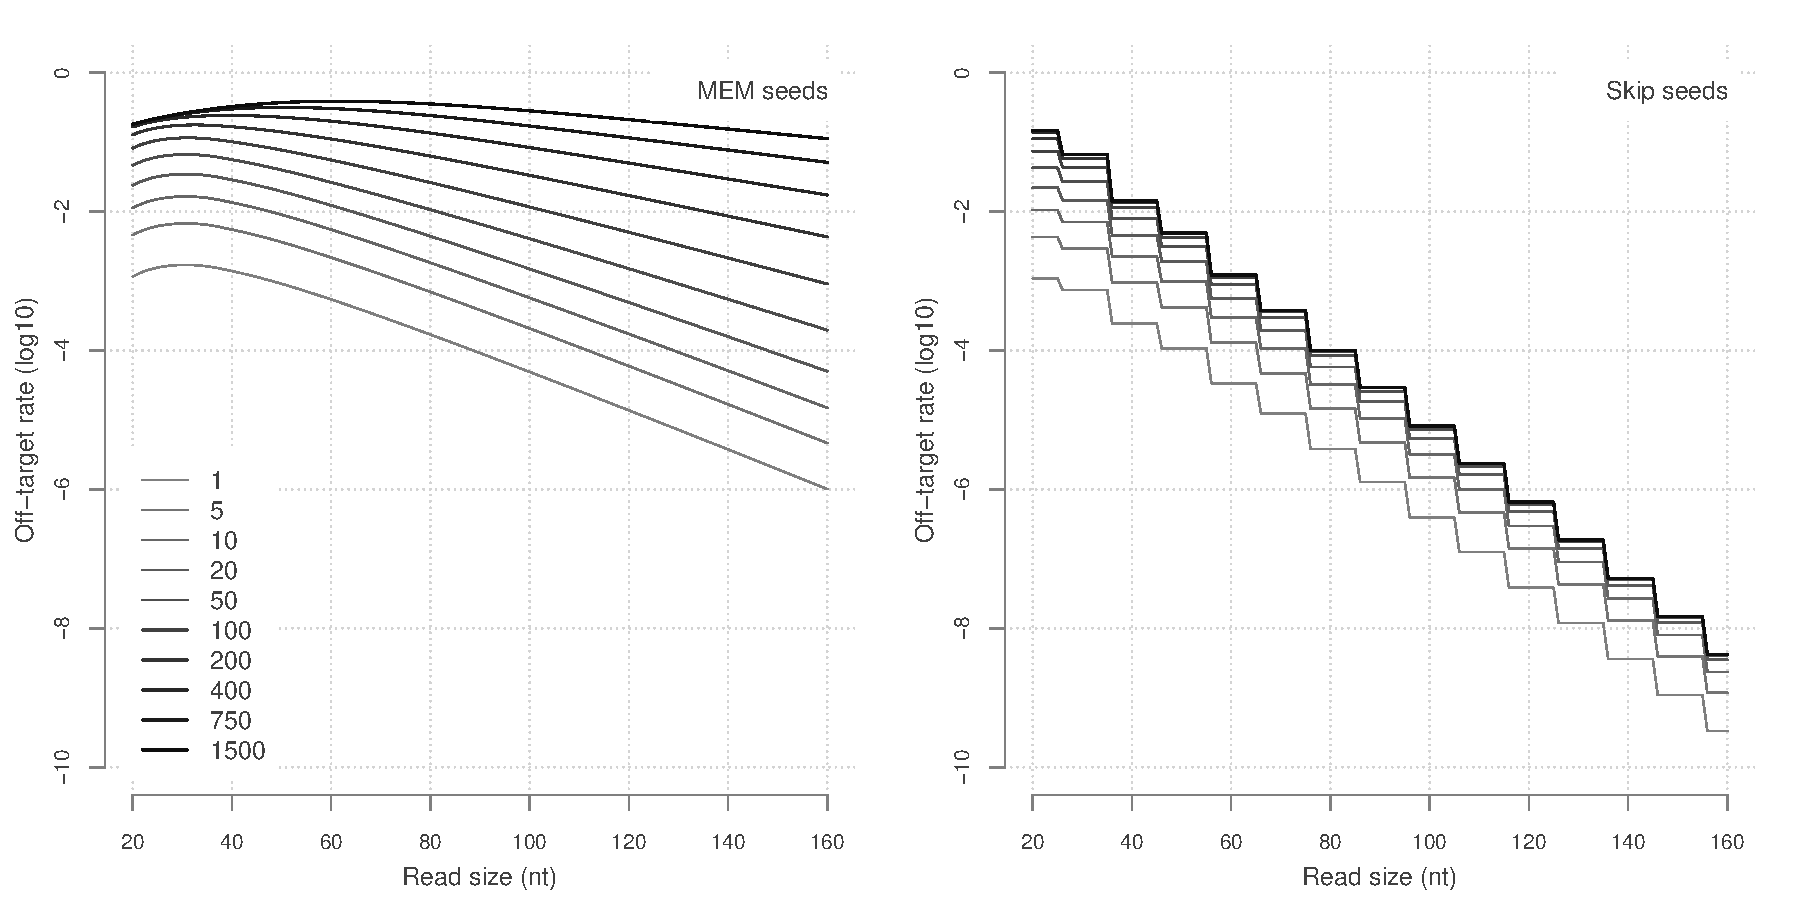
\includegraphics[scale=.6]{mortal_kombat.pdf}
\end{center}
\caption{Caption for wide figure over two columns.
\textbf{(a)} Left figure.
\textbf{(b)} Right figure (see (a)).
}
\label{fig_mortal_kombat}
\end{figure*}

Figure~\ref{fig_mortal_kombat} shows the off-target probabilities computed
by Sesame. Counter-intuitively, the probability initially increases with
the read size for MEM seeds. It turns out that off-target MEM seeds are
common in short reads that contain errors. Since longer reads have a
higher chance of containing an error, the off-target rate initially
increases. This effect dampens so that all the probabilities eventually
decrease exponentially, albeit at different rates.

For skip seeds, the off-target rates decrease in staircase with a drop
every 10 nucleotides. Indeed, the seeds are exactly the same if the read
length stays within the same decade. The curves show an overal linear
trend and have the same asymptotic rate.

From this we draw the important conclusion that the performance of skip
seeds degrades much less than MEM seeds when the target contains
paralogues. Skip seeds are thus better suited for sensitive mapping in
repeated sequences. Incidentally, this Figure~\ref{fig_mortal_kombat}
shows that it is suboptimal for a MEM-based mapper to all the candidate
loci when there is more than a handful of them: if the target has more
than 20 paralogues, the mapping quality will remain low even when the
output is correct. A better strategy is to either bail out or switch to a
more sensitive seeding method (BWA uses a re-seeding policy).

A related observation is that for MEM seeds, the off-target rate is above
$10^{-3}$ for reads of 50 nucleotides or less, meaning that beating
quality 30 is not straightforward in these conditions. It is important to
remember that mapping cannot be wrong if the target has no paralogue
(because it is trivial to recognize that false positives have no homology
with the read). Therefore, the main strategy to reach high mapping
confidence with MEM seeds is not to reduce the minimum seed size, but to
ascertain that the target is a unique sequence. We will show how to do
achieve this below.

Figure~\ref{fig_mortal_kombat} suggests that the performance of skip seeds
is better than that of MEM seeds. However one has to bear in mind that we
compare MEM seeds of size 19 with skip seeds of size 16: the gain in
sensitivity comes at the cost of a larger candidate set. In practice such
a large candidate set must be further filtered (Bowtie2 does this with a
priority policy), so the final performance of skip seeds cannot be as high
as suggested in the figure because of speed constraints.


\subsection{Estimating $N$ and $\mu$}
\label{ref_Nmu}

Estimating the two read-dependent parameters $N$ and $\mu$ is essential to
compute seeding probabilities. Recall that $N$ is the number paralogues of
the target ($N=0$ means that it is unique) and that $\mu$ is the sequence
divergence (the average fraction of mismatches between a paralogue and the
target).

The key observation is that the seeding algorithm can also reveal the
paralogue structure of the target. Queries in the FM index are carried out
using an algorithm known as the backward search. Extending the query one
nucleotide at a time, the backward search returns the number of matching
sequences in the genome. The decaying number of hits depends on how many
paralogues of the target are present in the genome, and how similar they
are with each other. It is thus possible to use the series of the backward
search to estimate $N$ and $\mu$.

Writing the likelihood of the process is straightforward if we assume that
nucleotides are used uniformly at random in the genome. The difficulty is
that the first iterations of the backward search are uninformative. For
instance, a query of length 10 is expected to have $\geq 3000$ hits in
the genome, so the potential paralogues of the target are hidden among so
many random hits. In practice, we ignore the first iterations until the
number of random hits is lower than 1. The information is labelled as
missing and the likelihood is updated accordingly. This gives a function
that can now by maximized with respect to $N$ and $\mu$.

Initial simulations revealed that the maximum likelihood estimates of $N$
and $\mu$ have a large variance. To mitigate this effect, we opted for a
grid search where we test only plausible values of $\mu$ and compute the
associated $N$ (see Methods). This gave a fast algorithm forced to produce
reasonable estimates.

We initially tested this method on the read, gathering the series of decay
during the seeding process. However, we quickly realized that this method
routinely missed paralogues because of sequencing errors. Using mapping as
an error correction mechanism, we tested a prototype estimating $N$ and
$\mu$ from the sequence of the best hit and obtained significantly better
results, so we settle for this option, even though it is slower. It is of
course possible that the best hit is not the target, but if it is a
paralogue, the estimated values of $N$ and $\mu$ should be similar.

\begin{figure*}[t]
\begin{center}
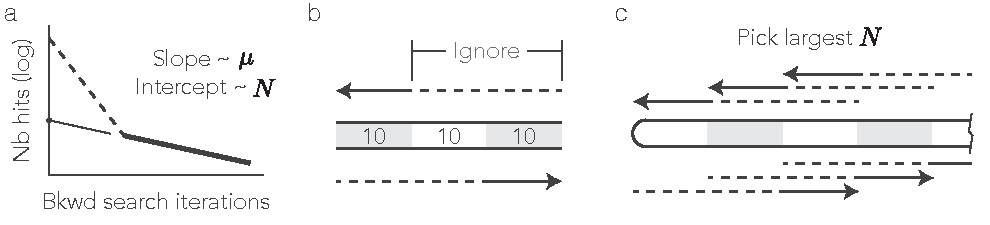
\includegraphics{strategy.pdf}
\end{center}
\caption{Caption for wide figure over two columns.
\textbf{(a)} Left figure.
\textbf{(b)} Right figure (see (a)).
}
\label{fig_strategy}
\end{figure*}

The estimation strategy is depicted in Figure~\ref{fig_strategy}. The
putative target is segmented in windows of 30 nucleotides overlapping by
20 nucleotides. The grid search is run a every window in both the foward
and reverse orientation, ignoring the first 20 iterations of the backward
search. The windowing approach accomodates the fact that only some
regions of the target may be repeated (e.g., if the read straddles a
transposon). Finally, we take the median values of $N$ and $\mu$ as
representative for the whole sequence.


\subsection{Super reads}
\label{sec_super}

While testing the estimation algorithm on reads of size 50, we observed
that a sub-population of them had mapping error rates below $10^{-5}$.
This is surprising in regard of Figure~\ref{fig_mortal_kombat}a because in
a genome where half of the sequences are duplicated, the error rate should
be $\approx 1/2 10^{-3}$. We reasoned that non-repeated sequences must be
overrepresented in this sub-population of reads.

Those reads are characterized by two facts: $i.$ they can be mapped witout
mismatch and $ii.$ the backward search depicted in
Figure~\ref{fig_strategy} retrieved only one sequence on each window.
Individually, these conditions are not uncommon among mapping errors, but
together they are exceedingly rare. Indeed, for a mapping error to occur,
the target must have a paralogue, the read must be identical to the
paralogue and the target must have been missed entirely while estimating
$N$ and $\mu$.

\begin{figure}[t]
\begin{center}
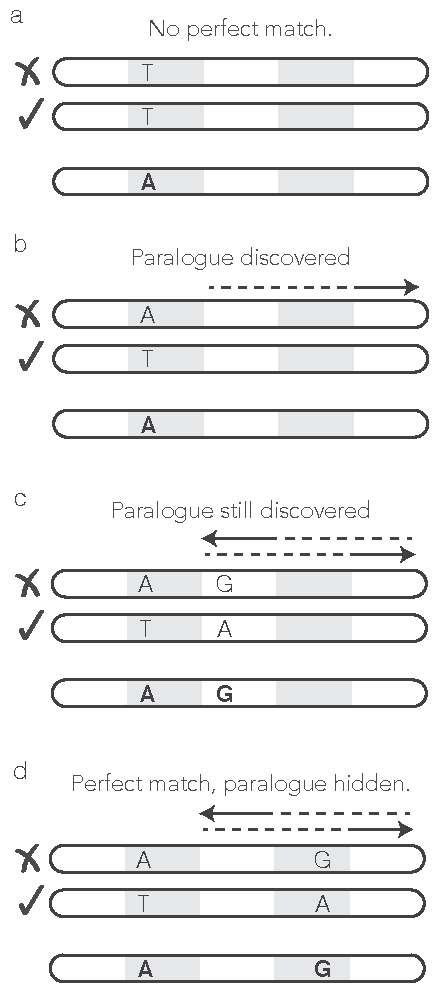
\includegraphics{super_reads.pdf}
\end{center}
\caption{Caption for figure within column.}
\label{fig_super}
\end{figure}

As shown in Figure~\ref{fig_super}, the most likely scenario for a
mapping error requires not just one, but two sequencing errors that match
the paralogue exactly. In addition, these errors must be at specific
positions of the read to mask the target. All other scenarios are even
less likely, making conditions $i.$ and $ii.$ strong features of
high-confidence mapping. Interestingly, those conditions are met on a
substantial fraction of reads because the error rate is typically around
1\% on short reads and 30-50\% of the sequences are unique in large
eukaryotic genomes.

Similar but more complex conditions hold when the read has 1 or 2
mismatches against the best hit, so that it is often possible to reach
high-confidence mapping when the target has no paralogue. Using such
techniques, it is possible to map 50 bp reads with quality 70 in realistic
sequencing conditions. This corresponds to one error in 10 million reads,
i.e. at most handful per sequencing run. For longer reads, the maximum
quality keeps increasing, but above 90 the differences become symbolic
because the chances of observing a mapping error in a whole project become
negligible.

As commented earlier, mapping errors cannot occur if the target has no
paralogue, so the key of super reads is to leverage the evidence that the
target is a unique sequence. This depends on the knowledge of the
reference genome, so the estimations are off on poorly assembled genomes.


\subsection{Implementing a mapper}

To evaluate the benefit of faithful mapping, we implemented a simple
mapper using Sesame. The mapping policy is to extracts MEM seeds of size
17 or more and to find the best scoring hit among the candidate loci by
Needleman-Wunsch alignment\cite{1}. The only exception is that the mapper
bails out if a MEM seeds has 300 or more hits in the genome, in which case
it returns a candidate at random. This approach is exceptionally naive in
comparison to modern mappers because it does not involve any refinement of
the candidate set, using for instance seed chainig or re-seeding. But once
the best candidate is found, the mapper estimates $N$ and $\mu$ using the
procedure described in section~\ref{sec_Nmu} and computes the mapping
quality with Sesame.

We measured the performance of this strategy on the genomes of increasing
complexity: \textit{Drosophila melanogaster} (the fruit fly), \textit{homo
sapiens} (modern humans) and \textit{Pinus taeda} (a north-American
species of pine). The basic features of the three genomes are summarized
in Table~\ref{table_genomes}. Fly and human are model organisms with
top-quality genome assembly. Pine is a non-model organism with a very
large and complex genome. We used BWA MEM and Bowtie2 with default
parameters to establish a baseline. The purpose of this benchmark is to
evaluate the feasability of the strategy outlined above and not to
advertise our prototype; it thus seemed inapropriate to run a
comprehensive survey of all the availble options of each mapper.

\begin{table}[b]
\tableparts{%
\caption{This is a table caption}
\label{table_genomes}%
}{%
\begin{tabular*}{\columnwidth}{@{}llrr}
\toprule
Organism & Reference & Size (Gbp) & Sequences \\
\colrule
\textit{D. melanogaster} & dm4/R6 & 0.15 & 1,870 \\
\textit{H. sapiens} & hg38/GRCh38 & 3.27 & 455 \\
\textit{P. taeda} & GCA\_000404065.3 & 22.50 & 1,760,464 \\
\botrule
\end{tabular*}%
}
{This is a table footnote}
\end{table}

We did not pay any particular attention to the memory footpring of the
mapper. Figure~\ref{fig_XX}a shows that the peak memory footprint is
approximately twice as large as that of BWA and Bowtie2. One of the
largest components of the FM index is the suffix array, which is
compressed by a factor 32 in the case of BWA and Bowtie2 versus 16 in the
case of our mapper. The reason for this choice is that the average memory
on modern workstations has more than doubled since the release of BWA MEM
and Bowtie2 around 2012, so we opted for an affordable boost in speed.

Figure~\ref{fig_XX}b shows that the speed of our prototype mapper was in
the same ballpark as that of BWA MEM and Bowtie2. The implementation
compensates for the simplicity of the mapping policy by prioritizing the
candidates loci, bailing out of the Needleman-Wunsch alignment as soon as
a candidate appears to be sub-optimal, or even skipping the alignment
whenever there is enough information at seeding stage to know that a
candidate cannot be the best hit. Estimating $N$ and $\mu$ takes
approximately x\% of the running time and computing probabilities with
Sesame is negligible. This shows that the time required to compute
accurate mapping qualities is not prohibitive and that faithful mapping is
compatible with the time constraints associated with short read mapping.

Having clarified this, our goal was of course to  evaluate the
faithfulness of the mappers on the different problems. We included
conditions far outside the expected, with error rates up to 10\%. The
intent here was to stress the mappers to evaluate the robustness of the
mappability scores. This is not entirely fair to BWA MEM and Bowtie2
because they are optimized for a lower error rate, whereas we provided the
error rate as a separate parameter for our mapper because it is required
by Sesame. Nevertheless, it is still interesting to know the behavior of
BWA MEM and Bowtie2 in stress conditions.

Figure~\ref{fig_YY} shows that our prototype mapper is faithful across all
conditions. For long reads, the mapping quality is underestimated in the
range below 20. Those reads map to repeated sequences where MEM seeds are
particularly inaccurate according to Figure~\ref{fig_mortal_kombat}. Yet,
this view appears to be somewhat pessimistic in practice. Yet, the true
mapping quality of those reads remains below 20 and qualifies as low
confidence in many applications.

Meanwhile, the faithfulness of BWA MEM and Bowtie2 is more variable and/or
biased. The quality scores estimated by BWA MEM are strictly ascending but
they are typically overstimated. For instance, the maximum quality 60 is
typically off by two orders of magnitude, even on model genomes in
realistc conditions. Still, the ascending nature of the score has two
significant benefits for the users: first they can re-calibrate the
quality scores by running simulations like this one, second they can be
sure that reads with a higher mapping quality scores are indeed more
likely to be correctly mapped. In comparison, the faithfulness profile of
Bowtie2 shows less bias and more variance. The claimed mapping quality is
overall in agreement with the empirical estimates, but the trend wiggles
up and down. It is more difficult for the user to re-calibrate the trend
or to select reads, but the benefit is that the claimed scores are
relatively close to their real value.

The maximum quality given by BWA MEM is 60 and that of Bowtie2 is 42. It
is not completely apparent from Figure~\ref{fig_YY} that our prototype
mapper goes much higher than either (the highest quality score in this
benchmark was XX). Importantly, these extreme mapping qualities are not
exaggerated: not a single read with quality above 60 is mapped at the
wrong location in the whole benchmark (this represents more than XX reads
without a single mistake). Those are mostly the super reads described in
section~\ref{sec_super} and they represent a significant benefit of using
Sesame.

Finally, it is important to see whether the gain in faithfulness comes at
the cost of accuracy. It is indeed questionable whether a MEM-based mapper
can achieve good accuracy without re-seeding. Figure~\ref{fig_ZZ} shows
that the overall accuracy of our prototype is comparable to that of BWA
MEM and Bowtie2. Note that it is possible to fine tune BWA MEM and Bowtie2
to reach higher accuracy (usually at the cost of computation time), but
once again our goal here is only to show that it is possible to achieve
faithfulness without sacrifices in speed or accuracy.

Overall, blah blah.


\section{DISCUSSION}

\subsection{Computational strategies for mapping quality}

Blah blah.

\subsection{SMMFDP and more}

The qualities of SMMFDP only come from faithfulness.

It is interesting to observe that the accuracy of BWA MEM and our
prototype are similar but they have entirely different origins. BWA MEM
uses re-seeding to increase the sensitivity of the heuristic and discover
candidates that escaped detection by MEM seeds. Our prototype gives up
relatively fast but through faithfulness it ranks the reads in a way that
optimizes the tradeoff.

Similarly, the speed of our prototype comes in part from not compressing
the suffix array as much as BWA MEM and Bowtie2, but more importantly from
not trying too hard to map difficult reads. The rationale is that reads
that are difficult to map end up with a poor mapping quality anyway, so
extra efforts have little benefit. That said, it is necessary at times to
push accuracy to its maximum and this strategy is inadapted. In such
cases, we would switch to a more sensitive seeding method, such as skip
seeds for instance, in order discover more candidates when there is
evidence that the target has paralogues in the genome. However, our
attempts with this strategy suggest that the benefit comes at a
significant cost of computational time.

\section{CONCLUSION}

It's awesome. 'Nough said.


\section{ACKNOWLEDGEMENTS}

We acknowledge the financial support of the Spanish Ministry of Economy,
Industry and Competitiveness (`Centro de Excelencia Severo Ochoa
2013-2017', Plan Nacional BFU2012-37168), of the CERCA
Programme~/~Generalitat de Catalunya, and of the European Research Council
(Synergy Grant 609989). R.~C. was supported by the People Programme
(Marie Curie Actions) of the European Union's Seventh Framework Programme
(FP7/2007-2013) under REA grant agreement 608959. We also acknowledge
support of the Spanish Ministry of Economy and Competitiveness (MEIC) to
the EMBL partnership.


\subsubsection{Conflict of interest statement.} None declared.
\newpage


\begin{thebibliography}{4}

% Format for article
\bibitem{1}
Author,A.B. and Author,C. (1992)
Article title.
\textit{Abbreviated Journal Name}, \textbf{5}, 300--330.

% Format for book
\bibitem{2}
Author,D., Author,E.F. and Author,G. (1995)
\textit{Book Title}.
Publisher Name, Publisher Address.

% Format for chapter in book
\bibitem{3}
Author,H. and Author,I. (2005)
Chapter title.
In
Editor,A. and Editor,B. (eds),
\textit{Book Title},
Publisher Name, Publisher Address,
pp.\ 60--80.

% Another article
\bibitem{4}
Author,Y. and Author,Z. (2002)
Article title.
\textit{Abbreviated Journal Name}, \textbf{53}, 500--520.

\end{thebibliography}

\end{document}
